\chapter{HC-PCA Confidence Regions}\label{chapter:HCPCA}

Although the limits of $H \times C$ are well defined, a complete characterization of its intrinsic topology is an open problem, due to the restrictions imposed by its curvilinear space.
The lack of knowledge of the joint distribution of the points obtained by this plane, due to the existing correlation between its variables, prevents the studies on test statistics for typical time series in this characterization space.
However, with the knowledge of the expected variability of such points, according to the underlying dynamics, we can test hypotheses for a wide variety of models.
Results in this direction can be found in the literature.
\cite{RandomNumberGeneratorsCausality} showed that the Complexity-Entropy plane ($ H \times C $) is a good indicator of the results of Diehard tests for pseudo-random number generators.
\cite{De_Micco_2008} evaluated ways to improve pseudo-random sequences for their representation in this plane.

In this context, a open problem present in the characterization of sequences using the $H \times C$ plane is the absence of a representative metric distance, which makes it difficult to build confidence regions.
Thus, in the proposed approach, we opted for the construction of empirical confidence regions obtained through an orthogonal projection of data in the space of principal components.
Therefore, the larger is the data set used to build the region, the more representative it will be.

To investigate the power of representation of the proposed confidence region, we defined as a first application a review of the results obtained in the literature using the $H \times C$ plane in pseudo-random sequences.
Thus, the necessary input to our algorithm consists of sequences of true random generated by physical procedures.
As a result, we verify how the sequences previously analyzed behaved in this new analysis scenario.

Below we list the main strategies and sequences analyzed by the literature for the study of randomness using the information theory descriptors.
Soon after, the test and characterization framework is presented.

\section{Complexity-Entropy plane in the literature}

The first works on the characterization of white noises with permutation entropy arose from the need to discriminate them in relation to chaotic maps~\citep{rosso2013characterization, xiong2020complexity}.

Stationary time series can be decomposed into two main components:
\begin{enumerate}
    \item \textbf{Deterministic}: it is described by a linear combination of its own past,
    \item \textbf{Random}: it is a component of the moving average of finite order.
\end{enumerate}
In this way, chaotic systems produce sequences composed of a physical structure, easily captured by measures of complexity.
Thus, it was found that the measure of statistical complexity was able to efficiently quantify the performance of pseudorandom number generators, expanding the possibilities of using information theory descriptors with the Bandt-Pompe symbolization~\citep{larrondo2002statistical, gonzalez2005statistical, RandomNumberGeneratorsCausality}.

Table~\ref{Tab:Literature} presents a summary of the main works in the literature that perform analysis of non-chaotic algorithmic generators, according to their features in $H \times C$.
We also provide the length $T$ and embedding dimension
$D$ of the time series under scrutiny. 
The following algorithmic generators were analyzed:
\begin{itemize}
    \item Mother RNG, available in Marsaglia website~\citep{marsaglia1994yet} (MOT);
    \item Multiple with carry RNG (MWC)~\citep{marsaglia1994yet};
    \item Combo RNG (COM)~\citep{marsaglia1994yet};
    \item Lehmer RNG (LEH)~\citep{payne1969coding};
    \item Fractional Gaussian noise with $\alpha = 0$ (fGn)~\citep{bardet2003generators};
    \item $f^{-k}$ noise with $k = 0$~\citep{larrondo2012matlab};
    \item Linear Congruential Generator (LCG)~\citep{knuth1997sorting}.
\end{itemize}

\begin{table}[htb]
    \caption{Result of the main works of white noise sequences analysis in the $H \times C$ plane.}
    \label{Tab:Literature}
    \centering
    \begin{tabular}{llccccb{5.4em}}
    \toprule
	Reference & PRNG & $T$ & $D$ & $H$ & $C$ & Considered random?\\ 
	\midrule
	\citeauthor{larrondo2013statistical} (\citeyear{larrondo2013statistical}) &  MOT & NA & 6 & $\cong 0.9969$ & $\cong 0$ & no\\
	\cmidrule(lr){1-7}
	\citeauthor{gonzalez2005statistical} (\citeyear{gonzalez2005statistical})  &  MWC & 65536 & NA & $\cong 1$ & $0.3$ & yes\\
	 &  MOT & 65536 & NA & $\cong 1$ & $0.3$ & yes\\
	 &  COM & 65536 & NA & $\cong 1$ & $0.05$ & yes\\
	\cmidrule(lr){1-7}
	\citeauthor{RandomNumberGeneratorsCausality} (\citeyear{RandomNumberGeneratorsCausality}) &  LEH & \num[scientific-notation=true]{5 e6} & 5 & $\cong 1$ & $10^{-4}$ & yes\\
	 &  MOT & \num[scientific-notation=true]{5 e6} & 5 & $\cong 1$ & $10^{-4}$ & yes\\
	 &  MWC & \num[scientific-notation=true]{5 e6} & 5 & $\cong 1$ & $10^{-4}$ & yes\\
	\cmidrule(lr){1-7}
	\citeauthor{rosso2013characterization} (\citeyear{rosso2013characterization}) &  LCG & \num[scientific-notation=true]{1 e7} & 6 & $0.997871$ & $0.005101$ & no\\
	\cmidrule(lr){1-7}
	\citeauthor{xiong2020complexity} (\citeyear{xiong2020complexity}) &  fGn & \num[scientific-notation=true]{2 e17} & 6 & $\cong 1$ & $\cong 0$ & yes\\
	 & $f^{-k}$ & \num[scientific-notation=true]{2 e17} & 6 & $\cong 1$ & $\cong 0$ & yes\\
	\bottomrule
    \end{tabular}
\end{table}

None of these works provide $p$-values or hypothesis tests for their analysis. 
The focus of the articles is finding the set of descriptors that best discriminates chaos from noise. 
The authors make assessments about the randomness of sequence on ad hoc visual inspection of the point’s location in the $H \times C$ plane. 
Our work fills such a gap for finite sequences of white noise and proposes a methodology that can be extended to any other situation.

\section{Proposed Method}

In this section, we formalize the task of building a confidence region in the Entropy-Complexity manifold.
Then, we present our proposal to change space through the algorithm of the principal components analysis.
Our goal is to find a latent space representative of the data, without the restrictions of a curvilinear space.
Through this new representation of the data, we calculate empirical regions with different levels of confidence.
Finally, after calculating these regions, we build a test statistic that determines the probability that a given sequence belongs to the distribution of the points provided.

\subsection{Overall Framework}

The structure of our proposal consists of two steps:
\begin{itemize}
    \item \textbf{Empirical confidence region}: With the data present in a Euclidean plane, we can easily calculate empirical regions that involve the data with a certain level of confidence.
    \item \textbf{Construction of a test statistic}: To measure the similarity of new data sequences with the empirical points, a test statistic was proposed. 
    By acquiring a p-value less than $0.05$, we can reject the null hypothesis, which states that such data belong to the empirical probability distribution used for the construction of the confidence region.
\end{itemize}

\subsection{Empirical Confidence Regions and \texorpdfstring{$p$}--values}\label{confidenceRegions}

Our first approaches to analyzing sequences of points in the $H\times C$ plane produced by TRWNS verified that they, and usual transformations, are far from bivariate Gaussian and generalized Hyperbolic distributions \citep{MultivariateDistributionModelswithGeneralizedHyperbolicMargins}.
Different types of regression models of $C$ explained by $H$ did not produce acceptable results.
Thus, we adopted a non-parametric approach and made an empirical analysis of the data obtained from physical sources for using them as our reference in the search for confidence regions and $p$-values.

Let $\utilde{x} =(x_1, x_2, \dots, x_N)$ be $N$ times series of length $T$, and define an embedding dimension $D$.
In the sequel, whenever possible, we will omit $T$ and $D$.
For each $n=1,2,\dots, N$, the time series $x_n$ is mapped onto the point $(h_n,c_n)$ in the $H\times C$ plane, thus $\utilde{hc}=\big((h_1,c_n), (h_2,c_2), \dots, (h_N,c_N)\big)$ are the points that correspond to the $N$ time series.
Fig.~\ref{fig:Methodology1} illustrates this step.
We will obtain confidence regions and $p$-values from $\utilde{hc}$.

The first step consists in finding and applying the principal components transformation to $\utilde{hc}$.
With this, we obtain the set of uncorrelated points $\utilde{uv}=\big((u_1,v_1), (u_2,v_2),\dots,(u_N,v_N)\big)$, in which $u_n$ and $v_n$ are the first and second principal components of $h_n$ and $v_n$, respectively.
This projection allows us to obtain a ``central'' point of the data set, around which we will build a rectangular box containing \SI{100}{\minusalphapercent} of the observations, where $\alpha$ is the significance level analyzed.
Such box is a variation of the bagplot \citep{TheBagplotaBivariateBoxplot}.
Notice that finding the smallest box that encloses $k$ out of $N$ points is difficult; cf.\ the work by \citet{SmallestKEnclosingRectangleRevisited}.

For simplicity, and without loss of generality, assume $N$ is odd.
\begin{enumerate}
	\item Find the indexes that sort the values of the first principal component $\bm u=(u_1,u_2,\dots,u_N)$ in ascending order: $\bm r=(r_1,r_2,\dots,r_N)$, i.e., $u_{r_1}$ is the minimum value, and $u_{r_N}$ is the maximum value.
	\item\label{item:Median} Find the point $(u,v)$ whose first principal component is the median: $(u_{r_{(N+1)/2}}, \cdot)$. Apply the inverse principal components transformation, and obtain $\bm P'=(h',v')$. Call the corresponding time series ``emblematic time series.''
	\item\label{item:Point1} Find the point $(u,v)$ whose first principal component is the quantile $\alpha/2$: $(u_{r_{[N\alpha/2]}}, \cdot)$.
	\item\label{item:Point2} Find the point $(u,v)$ whose first principal component is the quantile $1-\alpha/2$: $(u_{r_{[N(1-\alpha/2)]}}, \cdot)$.
	\item\label{item:Point3} The values $u_{r_{[N\alpha/2]}}$ and $u_{r_{[N(1-\alpha/2)]}}$ are the rightmost and leftmost bounds of the box, respectively.
	\item\label{item:Point4} The bottom bound of the box is the smallest second principal component value whose first principal component is at least $u_{r_{[N\alpha/2]}}$; denote this values $v_{\min}$.
	\item\label{item:Point5} The top bound of the box is the largest second principal value whose first principal component is at most $u_{r_{[N(1-\alpha/2)]}}$; denote this value $v_{\max}$.
	\item The corners of the box are 
	$(u_{r_{[N\alpha/2]}}, v_{\min})$, 
	$(u_{r_{[N\alpha/2]}}, v_{\max})$, 
	$(u_{r_{[N(1-\alpha/2)]}}, v_{\min})$ and 
	$(u_{r_{[N(1-\alpha/2)]}},v_{\max})$.
	\item\label{item:BoxHxC} Apply the inverse principal components transformation to these corners obtaining $\bm P_1=(h_{v_1}, c_{v_1})$, $\bm P_2=(h_{v_2},h_{v_2})$, $\bm P_3=(h_{v_3}, c_{v_3})$ and $\bm P_4=(h_{v_4},c_{v_4})$.
\end{enumerate}

Fig.~\ref{fig:methodology} illustrates these steps.
%
Fig.~\ref{fig:Methodology1} shows the points produced by TRWNS in the $H\times C$ plane.
The blue box includes a certain percentage of points, with sides parallel to the $H$ and $C$ axes.
The area in the $H\times C$ plane overestimates the desired proportion and may include ``unacceptable'' points.
%
Fig.~\ref{fig:Methodology2} shows the previous points projected onto the principal components space (steps~\ref{item:Median} to~\ref{item:Point5}).
The red box includes the same percentage of desired points, with axes parallel to the first and second principal components.
We highlighted in red the point whose first principal component is the median of the observed values.
%
Fig.~\ref{fig:Methodology3} shows the result of projecting back the red box from the principal components space to the $H\times C$ plane (step~\ref{item:BoxHxC}).
The comparison of the red and blue boxes shows that the area has been reduced, thus improving the test's power.

\begin{figure*}
	\centering
	\subfigure[Mapping true white noise random sequences onto the $H\times C$ plane.\label{fig:Methodology1}]{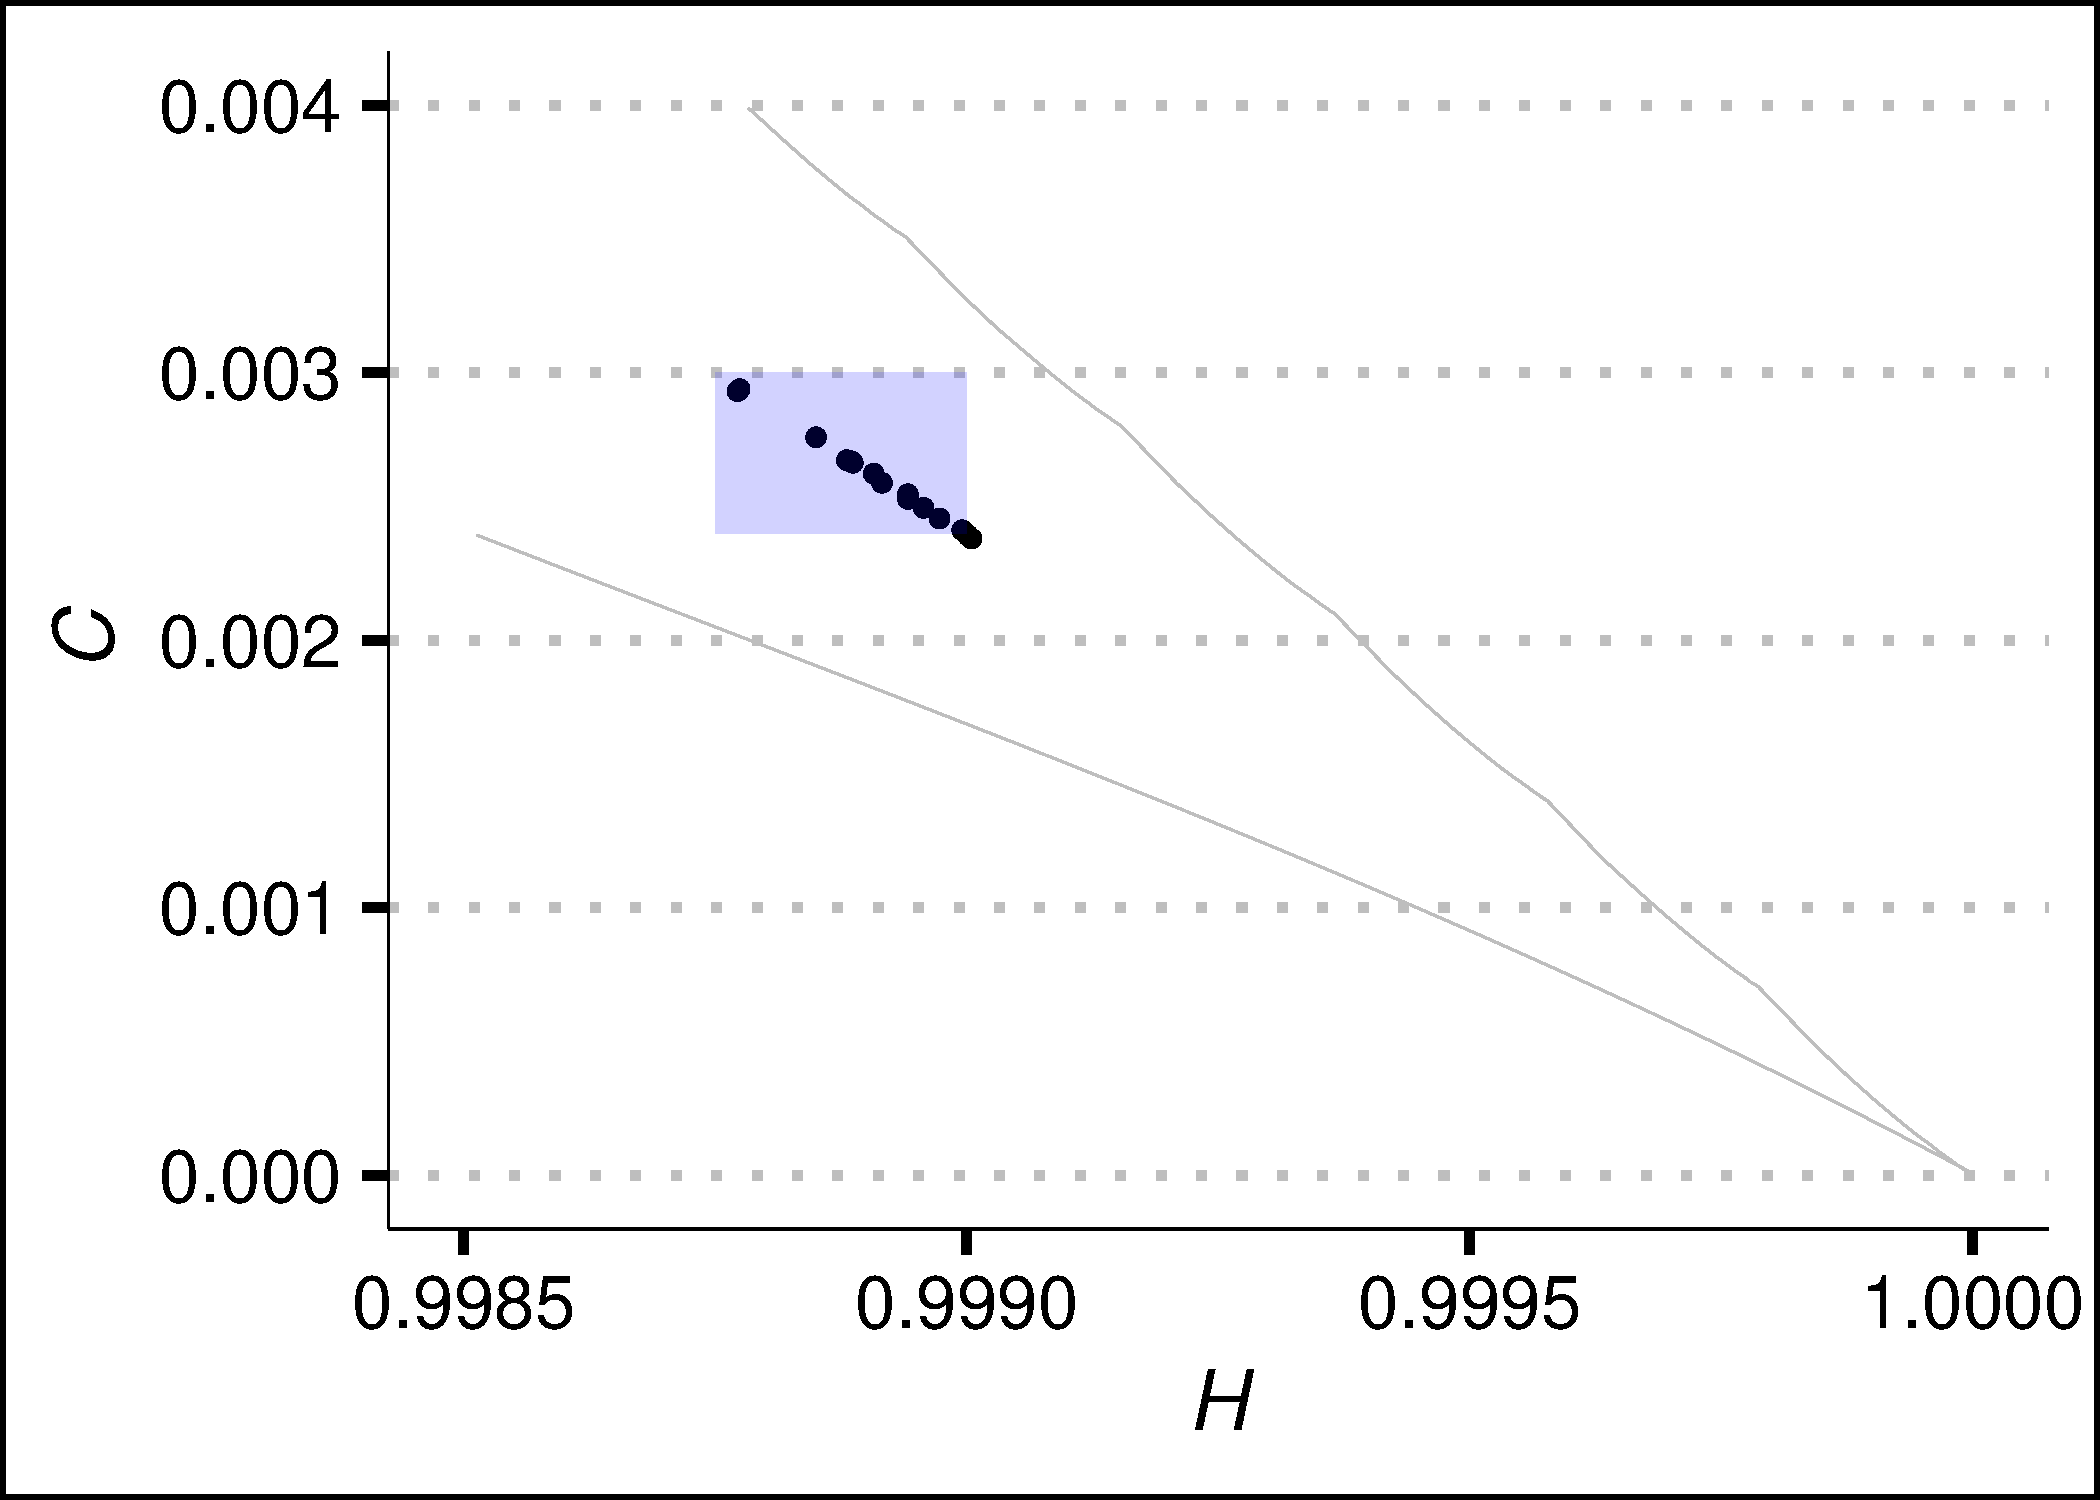
\includegraphics[width=.32\linewidth]{Figures/step1}}
	\subfigure[Transformation of the points in the $H\times C$ plane by Principal Components, and determination of minimal boxes.\label{fig:Methodology2}]{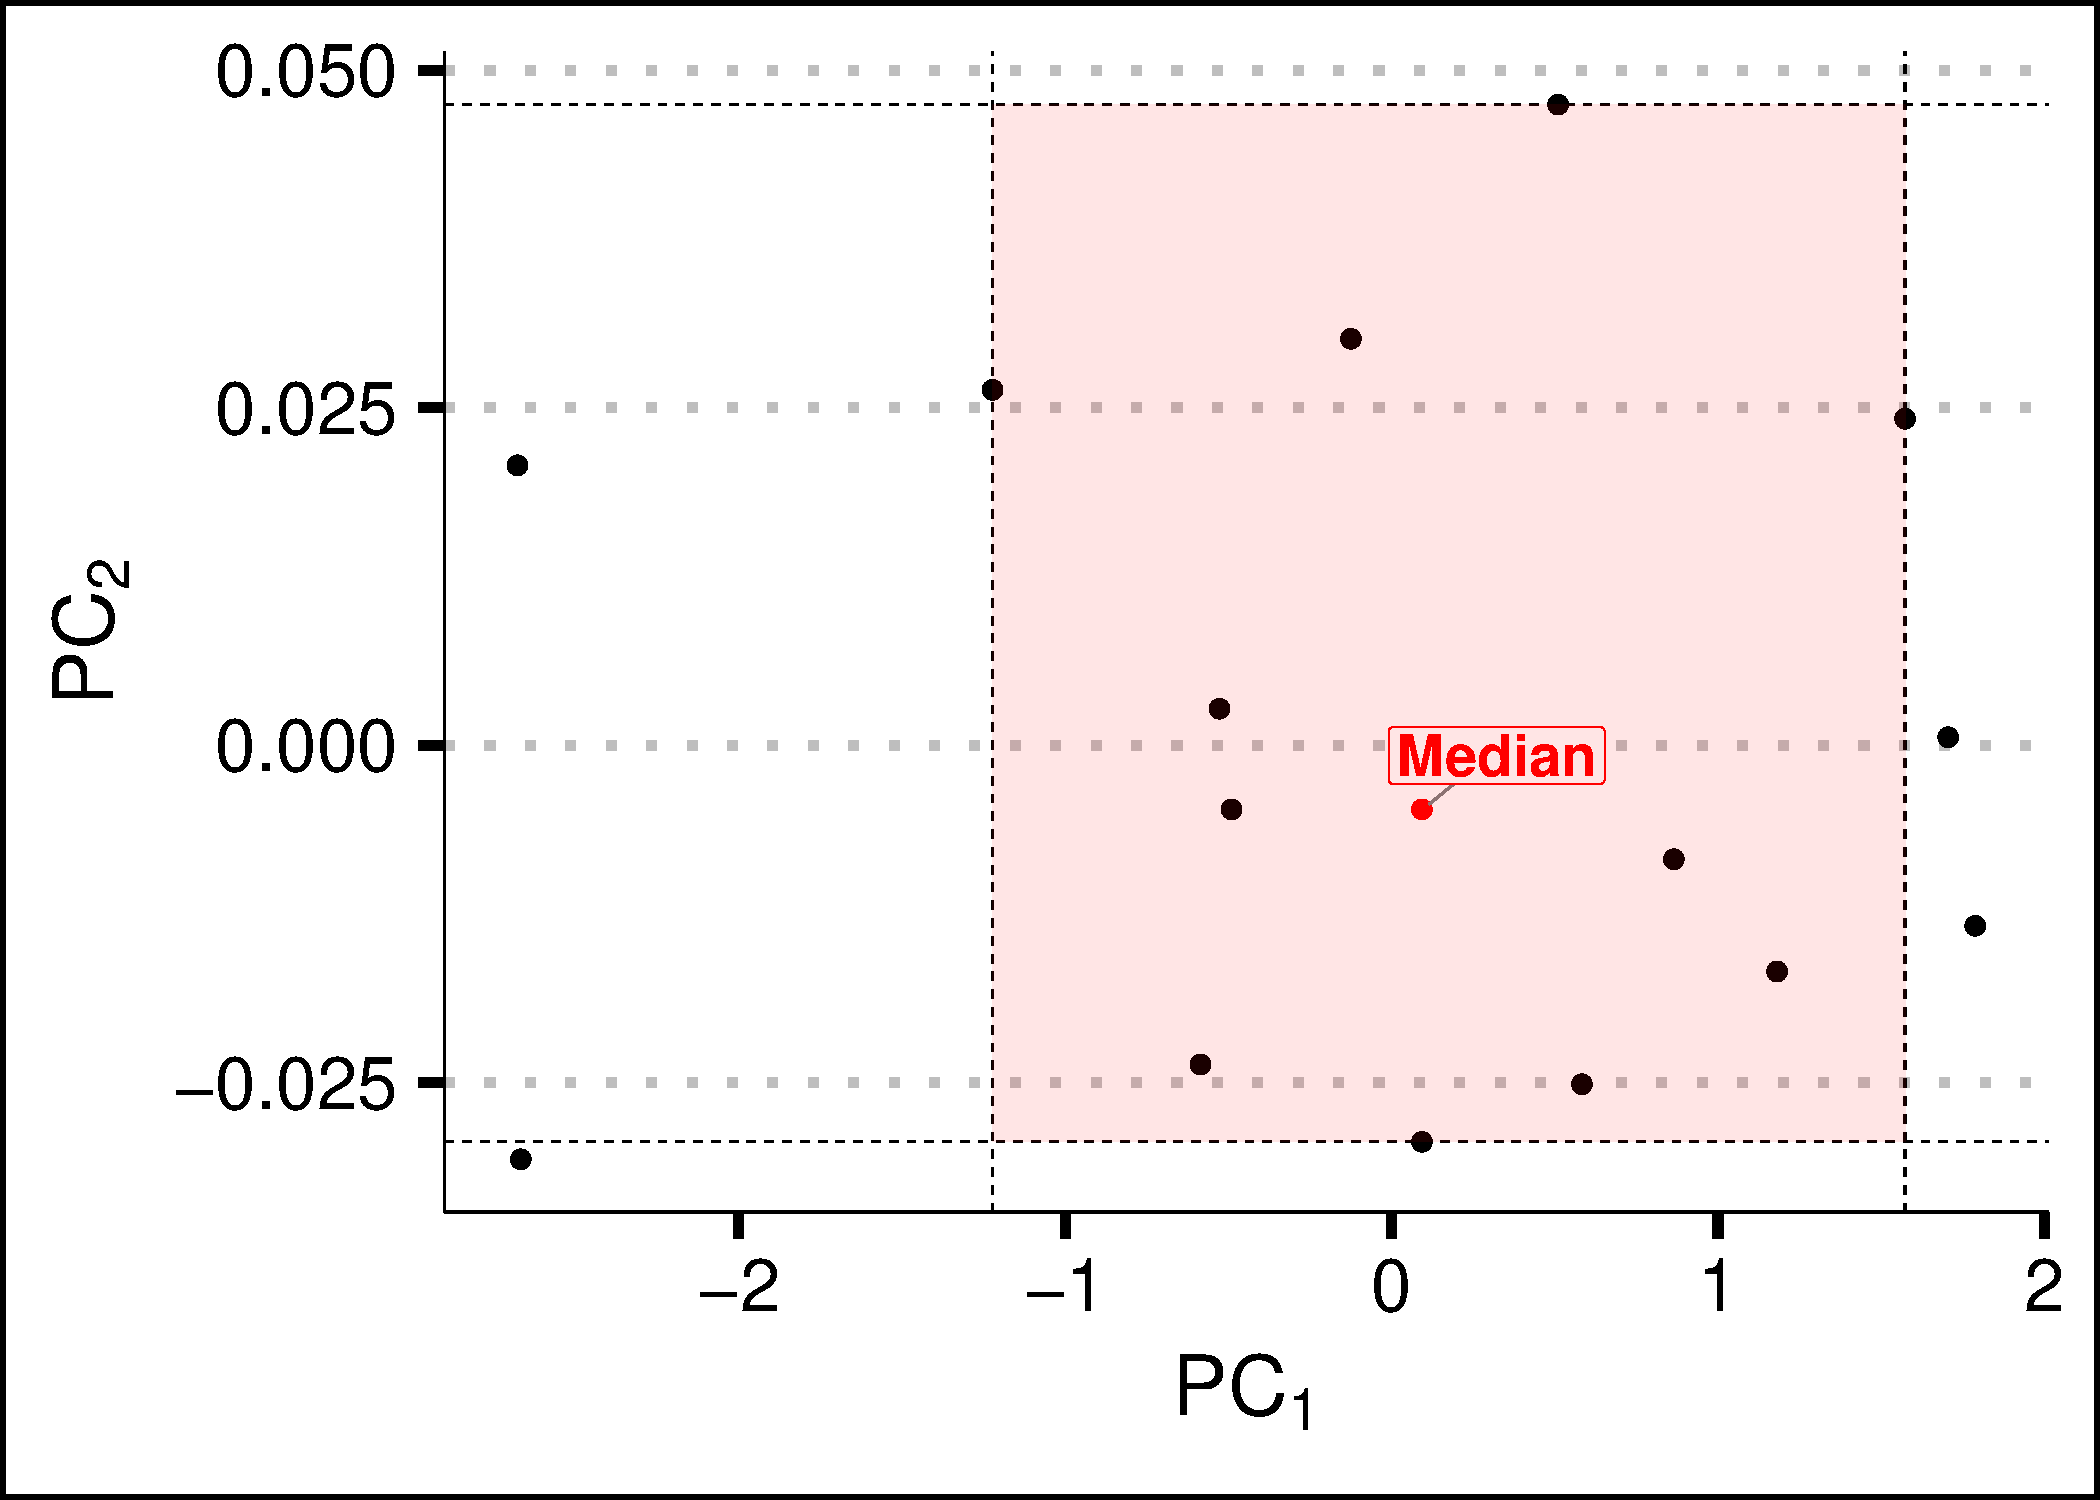
\includegraphics[width=.32\linewidth]{Figures/step2}}
	\subfigure[Inverse transformation from the Principal Components plane to the $H\times C$ plane.\label{fig:Methodology3}]{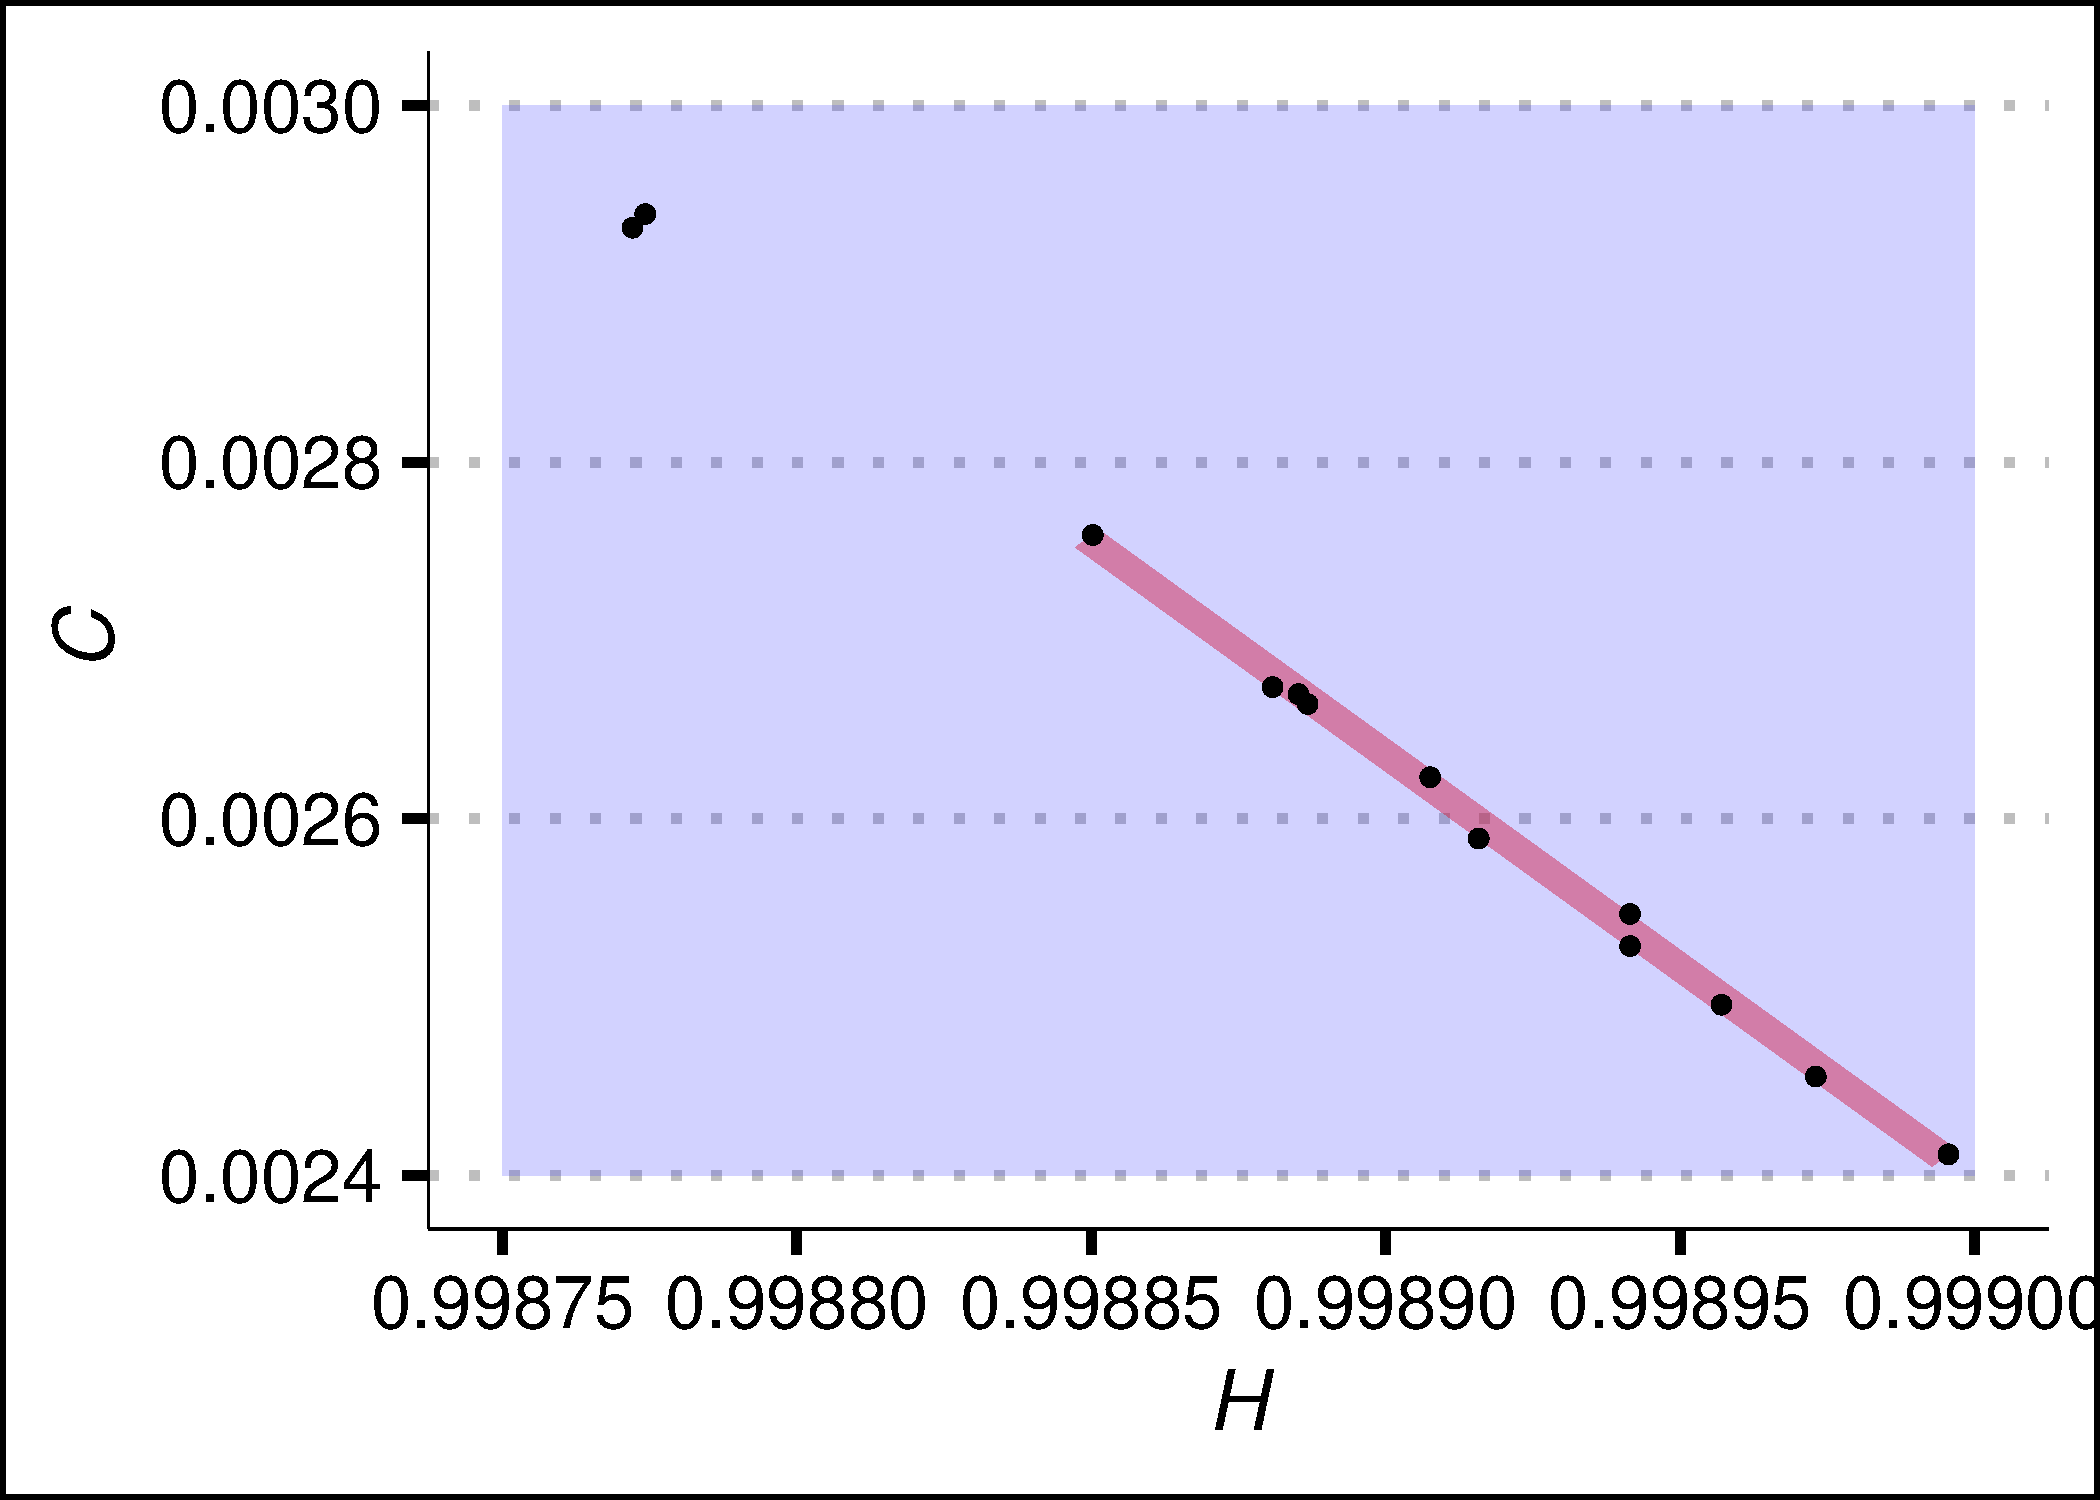
\includegraphics[width=.32\linewidth]{Figures/step3}}
	\caption{Outline of the methodology used for the construction of the confidence regions.}
	\label{fig:methodology}
\end{figure*}

Algorithm~\ref{Algo:ConfidenceRegions} provides details on how we obtain the confidence regions, defined by a set of points $\bm P_1, \bm P_2, \bm P_3, \bm P_4$, for each $D\in \mathcal D$, each $T\in \mathcal T$, and each significance level $\alpha$.
We also obtain the ``emblematic point'' $\bm P'$, a kind of median point in the $H\times C$ plane for each situation.


\begin{algorithm}[hbt]
	\SetKwInOut{Input}{input}\SetKwInOut{Output}{output}
	\Input{A data base of true random values}
	\Input{The desired values of embedding dimension $\mathcal D$, sequence length $\mathcal T$, and confidence levels $\mathcal A$}
	\Output{Confidence regions as points in the $H\times C$ plane}
	\For{each $D\in \mathcal D$}{
		\For{each $T\in \mathcal T$}{
			\For{each $n=1,2,\dots,N$}{
				build the time series $p_n$ with unused values from the data base\;
				compute the point $(h_n,c_n)$ in the $H\times C$ plane that corresponds to $p_n$\; 
			}
			obtain $\text{PC}(D,T)$, the principal components transformation based on the points $(h_1,c_1),(h_2,c_2),\dots,(h_N,c_N)$, and its inverse $\text{PC}^{-1}(D,T)$\;
			%
			apply $\text{PC}(D,T)$ to the points $(h_1,c_1),(h_2,c_2),\dots,(h_N,c_N)$, and obtain $(u_1,v_1),(u_2,v_2),\dots,(u_N,v_N)$\;
			%
			find the indexes $\bm r=(r_1,r_2,\dots,r_N)$ that sort the values of the first principal component $\bm u=(u_1,u_2,\dots,u_N)$ in ascending order\;
			%
			find the point $(u,v)$ whose first principal component is the median: $(u_{r_{(N+1)/2}}, \cdot)$\;
			%
			apply the inverse principal components transformation $\text{PC}^{-1}(D,T)$ to $(u,v)$, and obtain $\bm P'=(h',v')$; call the corresponding time series ``emblematic time series''\;
			\Return{$\bm P'$}\;
			%
			\For{each confidence level $\alpha \in \mathcal A$}{
				find the point $(u,v)$ whose first principal component is the quantile $\alpha/2$: $(u_{r_{[N\alpha/2]}}, \cdot)$\;
				%
				find the point $(u,v)$ whose first principal component is the quantile $1-\alpha/2$: $(u_{r_{[N(1-\alpha/2)]}}, \cdot)$\;
				%
				the values $u_{r_{[N\alpha/2]}}$ and $u_{r_{[N(1-\alpha/2)]}}$ are the rightmost and leftmost bounds of the box, respectively\;
				%
				the bottom bound of the box is the smallest second principal component value whose first principal component is at least $u_{r_{[N\alpha/2]}}$; denote this value $v_{\min}$\;
				%
				the top bound of the box is the largest second principal value whose first principal component is at most $u_{r_{[N(1-\alpha/2)]}}$; denote this value $v_{\max}$\;
				%
				the corners of the box are 
				$(u_{r_{[N\alpha/2]}}, v_{\min})$, 
				$(u_{r_{[N\alpha/2]}}, v_{\max})$, 
				$(u_{r_{[N(1-\alpha/2)]}}, v_{\min})$ and 
				$(u_{r_{[N(1-\alpha/2)]}},v_{\max})$\;
				%
				apply the inverse principal components transformation $\text{PC}^{-1}(D,T)$ to these corners obtaining $\bm P_1=(h_{v_1}, c_{v_1})$, $\bm P_2=(h_{v_2},h_{v_2})$, $\bm P_3=(h_{v_3}, c_{v_3})$ and $\bm P_4=(h_{v_4},c_{v_4})$\;
				\Return{$\bm P_1$, $\bm P_2$, $\bm P_3$, $\bm P_4$}\;
			}
		}
	}
	\caption{Determination of confidence regions and emblematic time series}
	\label{Algo:ConfidenceRegions}
\end{algorithm}

These confidence regions obtained provide a powerful tool to make binary assessments about the adequacy of a given time series $\bm x$ to the null hypothesis $\mathcal H_0$ that it is white noise.
More generally, we are interested in obtaining the $p$-value of $\bm x$ under $\mathcal H_0$.
We present a procedure to obtain an approximate $p$-value based on the evidence collected to build the confidence regions.

The procedure operates on the principal components space and consists of measuring the closeness between the ``emblematic point'' and the observed point.
We are given a time series $\bm x$ of size $T$, and we want its $p$-value when contrasted with TWNRS of the same size at embedding dimension $D$.
We use $N$ TWNRS of size $T$, compute their points in the $H\times C$ plane, and project them to the corresponding principal components space.
We then do the same with $\bm x$, and obtain a new point $(u_x,v_x)$.
The closer $\bm x$ is to the emblematic time series, the larger its $p$-value.
Assume that the emblematic time series is represented by $(u,v)$ in the principal components space.
We measure this closeness by building a box around $(u_x,v_x)$ that contains $(u,v)$; assume that $u_x>u$, then:
\begin{enumerate}
	\item the right side of the box is the smallest $u_j$ which is larger that $u_x$; assume it corresponds to the quantile $\eta_u$ of $\utilde u = (u_1,u_2,\dots, u_N)$. By definition, $\eta_u\geq 1/2$.
	%
	\item the left side of the box is the $1-\eta_u$ quantile of $\utilde u$.
	%
	\item the top side of the box is the smallest $v_j$ which is larger that $v_x$; assume it corresponds to the quantile $\eta_v$ of $\utilde v = (v_1,v_2,\dots, v_N)$. By definition, $\eta_v\geq 1/2$.
	%
	\item the bottom side of the box is the $1-\eta_v$ quantile of $\utilde v$.
\end{enumerate}
Fig.~\ref{fig:methodologyPvalue} illustrates theses steps.

The definition of the box for the case $u_x<u$ follows naturally, and is described in Algorithm~\ref{Algo:p-value}.
With this approach, we obtain the smallest box that (i)~contains the new point, and (ii)~is defined by observed points from TRWNS.

Such boxes are less prone to distortions in this space since the distribution of the points becomes less asymmetric than in the $H\times C$ plane; cf.\ Fig.~\ref{fig:HC-PCA}.
Algorithm~\ref{Algo:p-value} shows the details.

\begin{figure*}
	\centering
	\subfigure[Points produced by TRWNSs in the space of principal components.\label{fig:v1}]{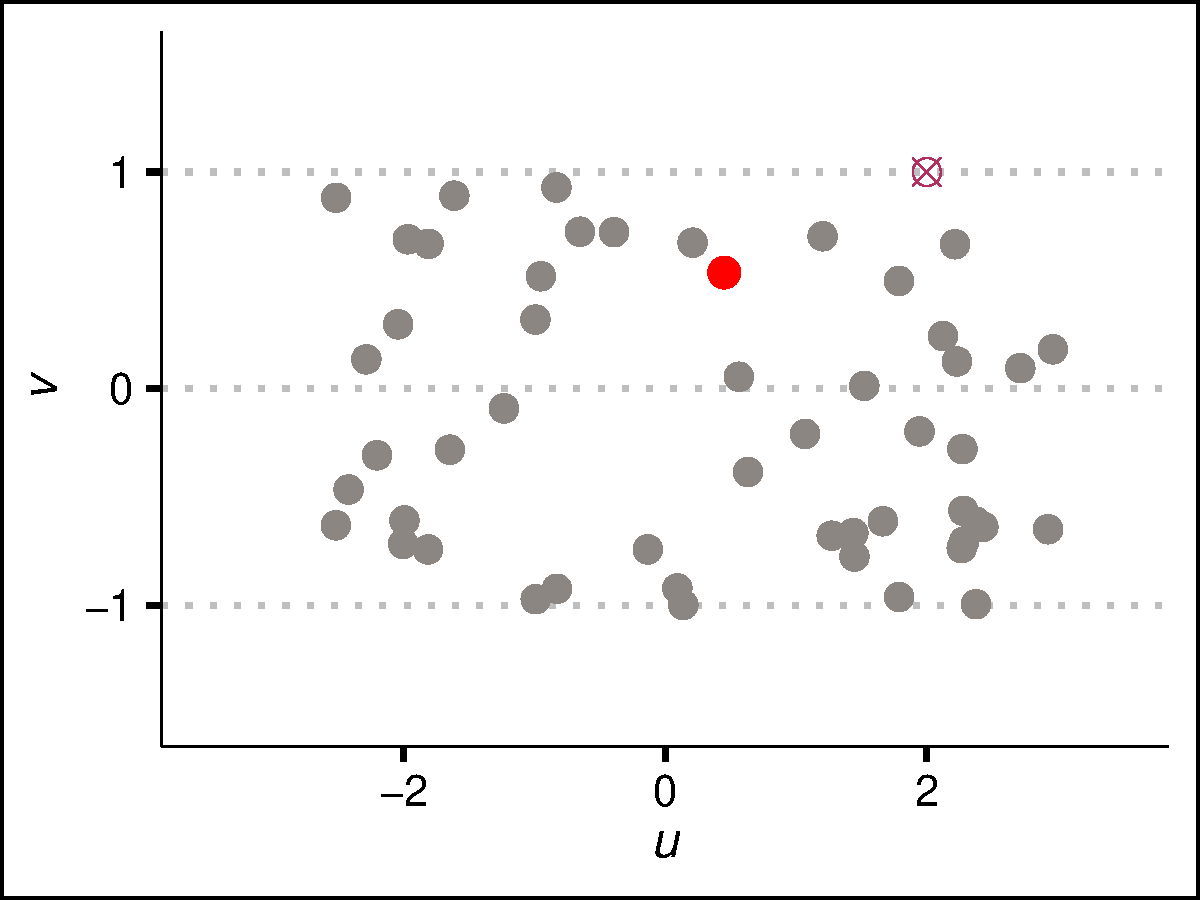
\includegraphics[width=.325\linewidth]{Figures/PvalueStep1}}
	\subfigure[Points whose first principal component is the median (red) and quantiles of order $\eta_u$ and $1-\eta_u$ (green).\label{fig:methodologyPvalue2}]{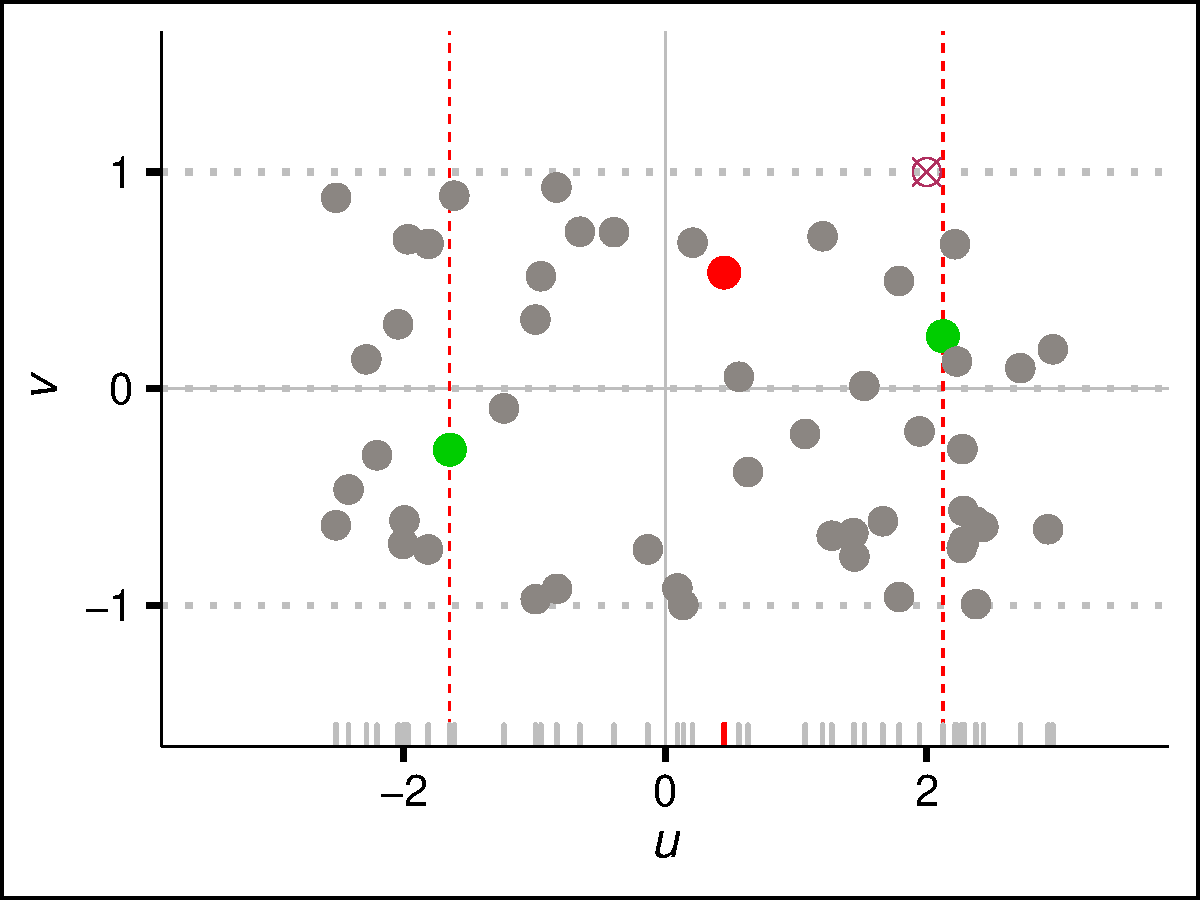
\includegraphics[width=.325\linewidth]{Figures/PvalueStep2}}
	\subfigure[The $p$-value of the new point is the proportion of points outside the box.\label{fig:methodologyPvalue3}]{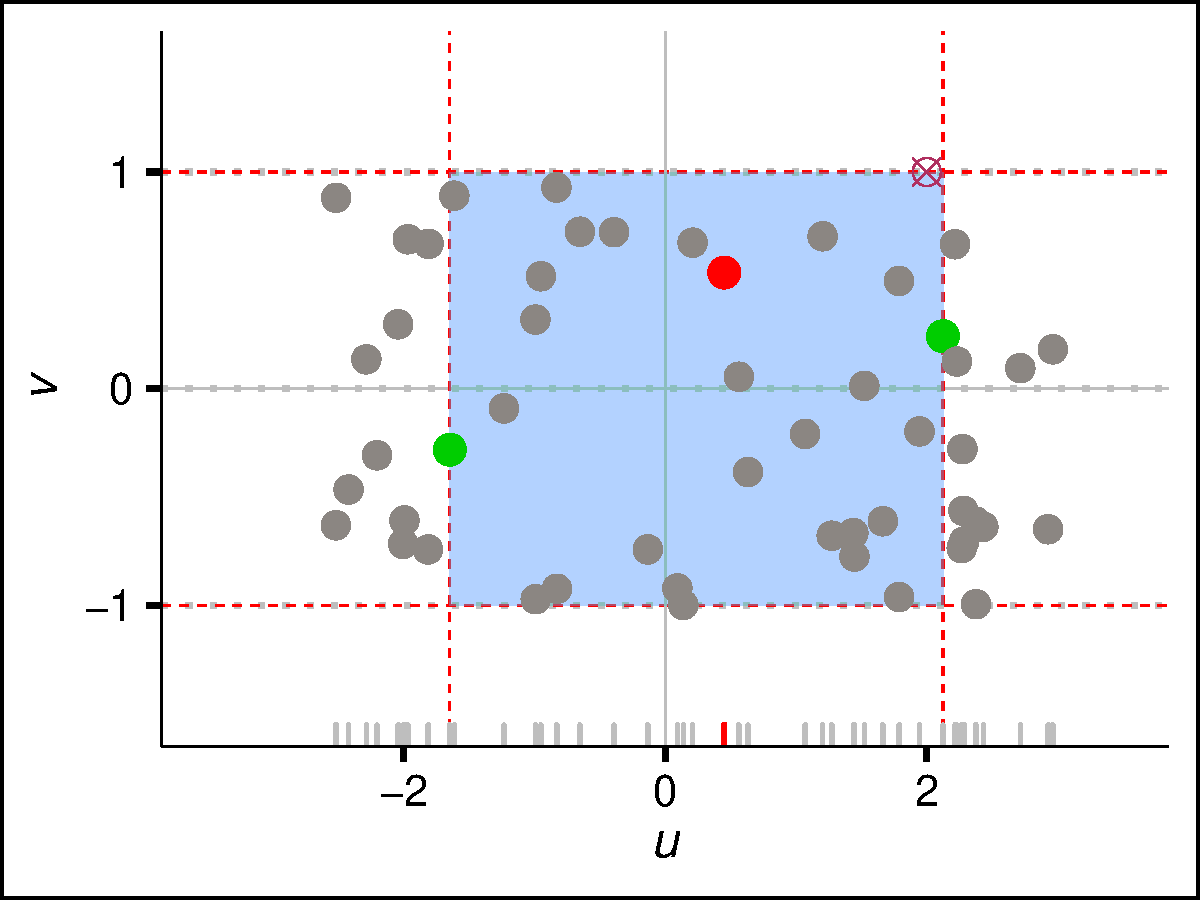
\includegraphics[width=.325\linewidth]{Figures/PvalueStep3}}
	\caption{Outline of the methodology used to calculate the $p$-value. The new point is denoted as a crossed circle.}
	\label{fig:methodologyPvalue}
\end{figure*}

\begin{algorithm}[hbt]
	\SetKwInOut{Input}{input}\SetKwInOut{Output}{output}
	\Input{The sequence $\bm x$ of length $T$ to be contrasted to the null hypothesis $\mathcal H_0$ that it is adherent to white noise}
	\Input{The embedding dimension $D$}
	\Input{$N$ points $(h_1,c_1),(h_2,c_2),\dots,(h_N,c_N)$ of true white noise series of length $T$;
		the principal components tranformation $\text{PC}(D,T)$ induced by these points;	
		the points projected onto the $H\times C$ plane: $(u_1,v_1),(u_2,v_2),\dots,(u_N,v_N)$}
	\Output{An approximate $p$-value}
	find the point $(u,v)$ whose first principal component is the median: $(u_{r_{(N+1)/2}}, \cdot)$\;
	find the point $(h,c)$ of the sequence $\bm x$\;
	find the projection $(u_x,v_x)$ of $(h,c)$ onto the principal components space using $\text{PC}(D,T)$\;	
	\eIf{$u_x > u$}
	{ $u_{r_{[N(1-\alpha/2)]}}$ is defined as the smallest element larger than $u_x$\;
		$u_{r_{[N\alpha/2]}} \leftarrow 2u - u_{r_{[N(1-\alpha/2)]}}$\;
	}
	{
		\eIf{$u_x < u$}
		{ $u_{r_{[N\alpha/2]}}$ is the largest minor element of $u_x$\;
			$u_{r_{[N(1-\alpha/2)]}} \leftarrow 2u - u_{r_{[N\alpha/2]}}$\;
		}
		{ $u_{r_{[N\alpha/2]}}$ and $u_{r_{[N(1-\alpha/2)]}}$ is equal to $u$, the median point of the first principal component\; 
		}
	}
	obtain the maximum values of the second component whose values of the first principal component are at least $u_{r_{[N\alpha/2]}}$ and at most $u_{r_{[N(1-\alpha/2)]}}$ and denote it $v_{\max}$\;
	obtain the minimum values of the second component whose values of the first principal component are at least $u_{r_{[N\alpha/2]}}$ and at most $u_{r_{[N(1-\alpha/2)]}}$ and denote it $v_{\min}$\;
	the corners of the box $b_{\alpha}(h,c)$ are 
	$(u_{r_{[N\alpha/2]}}, v_{\min})$, 
	$(u_{r_{[N\alpha/2]}}, v_{\max})$, 
	$(u_{r_{[N(1-\alpha/2)]}}, v_{\min})$ and 
	$(u_{r_{[N(1-\alpha/2)]}}, v_{\max})$\;
	%find $b_{T,D}(h,c)$: the smallest box centered at $(h',c')$ which contains $\text{PC}(D,T)(h,c)$\;
	count $n_{\bm x}$, the number of points out of the $N$ points which belong to $b_{\alpha}(h,c)$\;
	\Return{$1-n_{\bm x}/N$}
	\caption{Determination of the $p$-value of the sequence $\bm x$ under $\mathcal H_0$}\label{Algo:p-value}
\end{algorithm}

